\documentclass[12pt,a4paper,UTF8]{ctexart}

\usepackage{geometry}
    \geometry{left=2.5cm,right=2.5cm,top=2.2cm,bottom=2.8cm}

\usepackage{graphicx}
\usepackage{subfigure}
\usepackage{amsmath}
\usepackage{setspace}
\usepackage{enumitem}
\usepackage{mdframed}
\usepackage{everypage}
\usepackage{lastpage}
\usepackage{listings}
\usepackage{caption}
\usepackage{pifont}
\usepackage{diagbox}
\usepackage{pdfpages}

\usepackage{lipsum}

\usepackage{tikz}
\usetikzlibrary{calc}

\usepackage{draftwatermark}
\SetWatermarkText{Transcribed by Elricor}
\SetWatermarkScale{0.5}
\SetWatermarkLightness{0.75}

\usepackage{fancyhdr}
\pagestyle{fancy}
\lhead{中山大学《电子技术实验》预习报告}
\rfoot{\today}
%\renewcommand{\headrulewidth}{0pt}
\renewcommand{\theenumi}{(\arabic{enumi})}

\begin{document}

\AddEverypageHook{%
  \begin{tikzpicture}[remember picture,overlay]
    \draw[line width=1.2pt,rounded corners=0pt]
      ($(current page.north west)+(1.8cm,-1.4cm)$) rectangle ($(current page.south east)+(-1.8em,1cm)$);
  \end{tikzpicture}
}

\vspace{2em}
\begin{center}
    {\LARGE\bfseries 《电子技术实验》预习报告}

\end{center}
\vspace{2em}

\begin{doublespace}
    \centering
    \begin{tabular}{c c c}
        学院：$\qquad \qquad \qquad \qquad$ & 专业：$\qquad \qquad \qquad \qquad$ & 年级：$\qquad \qquad \qquad \qquad$ \\
    \end{tabular}

\end{doublespace}

实验人姓名（学号）：

同组实验人姓名（学号）：

\begin{center}
    \underline{~~~~~~}年\underline{~~~~~~}月\underline{~~~~~~}日~~~~~~上午~~~下午~~~晚上
\end{center}

\noindent\rule{\textwidth}{0.8pt}

\vspace{1.8em}
\begin{center}
    {\large\bfseries 实验一~~~单级与反馈放大电路}

    （第一部分——三极管特性曲线的测量）
\end{center}

\renewcommand\thesubsection{1.\arabic{subsection}}
\setcounter{subsection}{0}
\subsection{输入特性曲线的测量}

\begin{figure}[h]
    \centering
    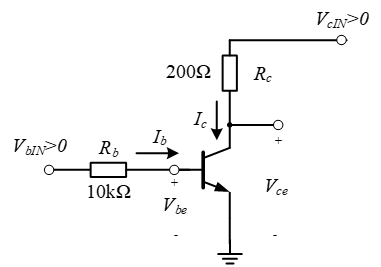
\includegraphics[width=0.5\textwidth]{电路图.png}
    \caption{输入特性曲线测量电路图}
    \label{fig:电路图}
\end{figure}

\begin{enumerate}[label=(\arabic*)]
    \item 按照电路图仔细连接实验电路，确保各元器件和导线连接正确无误。连接完成后，逐一检查各连接点是否牢固，避免虚焊或接触不良。确认无误后，缓慢接通电源，观察电路有无异常现象（如元件发热、异味等），确保实验安全。

    \item 缓慢调节输入电压$V_{bIN}$，每次调节时注意电压变化的幅度，避免过快或过大。分别在不同的$V_{bIN}$下，使用万用表或实验仪器准确测量并记录$V_{be}$和$I_{b}$的数值。将每组测量数据认真填写在数据表中，注意单位和数值的准确性。

    \item 在不同的$V_{bIN}$下，重复上述测量步骤，尽量多测量几组数据，以覆盖更广的电压范围。每次测量后对比数据，检查是否存在异常或误差。通过多组数据的积累，确保实验结果的准确性和完整性，并初步观察输入特性曲线随$V_{bIN}$变化的趋势，为后续分析做准备。
\end{enumerate}

\begin{table}[h]
    \centering

    \begin{tabular}{|c|c|c|c|}
        \hline
        $V_{bIN} \left(\mathrm{mV}\right) $ 测试值 & $V_{bIN} \left(\mathrm{mV}\right) $ 测试值 & $V_{be} \left(\mathrm{mV}\right) $ 测试值 & $I_{b} \left(\mathrm{\mu V}\right)$ 计算值 \\ \hline
        0   & 0    & 0    & 0    \\ \hline
        50  & 50   & 480  & 0.1  \\ \hline
        100 & 100  & 520  & 0.3  \\ \hline
        150 & 150  & 560  & 0.7  \\ \hline
        200 & 200  & 600  & 1.2  \\ \hline
        250 & 250  & 630  & 2.0  \\ \hline
        300 & 300  & 650  & 3.1  \\ \hline
        350 & 350  & 670  & 4.5  \\ \hline
        400 & 400  & 680  & 6.0  \\ \hline
    \end{tabular}
    \caption{输入特性曲线测量数据表}
    \label{tab:input_characteristics}
\end{table}

\textbf{备注和补充数据：}
\lipsum[1]

\subsection{输出特性曲线的测量}
\lipsum[2]

\renewcommand\thesubsection{2.\arabic{subsection}}
\setcounter{subsection}{0}
\subsection{输入特性曲线的测量}
\lipsum[3]

\subsection{输出特性曲线的测量}

\lipsum[4]

%\end{mdframed}
\end{document}